\documentclass[a4paper, 12pt]{article}

\usepackage[utf8]{inputenc}
\usepackage[spanish]{babel}
\usepackage[margin=1.5in]{geometry}
\usepackage{graphicx}
\usepackage{float}
\usepackage{pdfpages}
\usepackage{listings}
\usepackage{listingsutf8}
\usepackage{xcolor}
\usepackage{scrextend}
\usepackage{array, multirow}
\usepackage{booktabs}
\usepackage{tabularx}

\definecolor{mGreen}{rgb}{0,0.6,0}
\definecolor{mGray}{rgb}{0.5,0.5,0.5}
\definecolor{mPurple}{rgb}{0.58,0,0.82}
\definecolor{backgroundColour}{rgb}{0.95,0.95,0.92}

\newcolumntype{C}[1]{>{\centering\arraybackslash}p{#1}}

\lstset{
language=C,
%backgroundcolor=\color{backgroundColour},   
commentstyle=\color{mGreen},
%keywordstyle=\color{magenta},
keywordstyle=\color{blue},
%numberstyle=\tiny\color{mGray},
stringstyle=\color{mPurple},
tabsize=4,
basicstyle=\fontsize{11}{13}\ttfamily\footnotesize,
showspaces=false,
showstringspaces=false,
captionpos=b,
breaklines=true
}


%\lstdefinestyle{CStyle}{
%    backgroundcolor=\color{backgroundColour},   
%    commentstyle=\color{mGreen},
%    keywordstyle=\color{magenta},
%    numberstyle=\tiny\color{mGray},
%    stringstyle=\color{mPurple},
%    basicstyle=\footnotesize,
%    breakatwhitespace=false,         
%    breaklines=true,                 
%    captionpos=b,                    
%    keepspaces=true,                 
%    numbers=left,                    
%    numbersep=5pt,                  
%    showspaces=false,                
%    showstringspaces=false,
%    showtabs=false,                  
%    tabsize=2,
%    language=C
%}


\title{		\textbf{Trabajo Práctico 1}\\
			\textbf{Conjunto de instrucciones MIPS}
			}

\author{	Lucas Medrano, \textit{Padrón Nro. 99247}                     	\\
            \texttt{ lucasmedrano97@gmail.com }                           		\\
            Federico Álvarez, \textit{Padrón Nro. 99266}                 	\\
            \texttt{ fede.alvarez1997@gmail.com }                                 	\\[2.5ex]
            \normalsize{Grupo Nro. \quad - 2do. Cuatrimestre de 2018}      	\\
            \normalsize{66.20 Organización de Computadoras}               	\\
            \normalsize{Facultad de Ingeniería, Universidad de Buenos Aires}\\
       }
\date{}

\begin{document}
	\lstset{inputencoding=utf8/latin1} % Incorpora acentos en los listings
	\maketitle
	\thispagestyle{empty}
	\begin{abstract}
		En este trabajo se quiere desarrollar un programa escrito en lenguaje C que implementa un algoritmo de Quicksort. Dicho programa ordena alfabéticamente o numéricamente las líneas de un archivo \texttt{.txt}. Se visualizará en pantalla tanto el resultado como los errores que se produzcan. El algoritmo de Quicksort tendrá una implementación en assembler MIPS32, además de la versión en C, para la cual se empleará la convención de pasaje de parámetros establecida en la ABI explicada en clase.
	\end{abstract}
	
	\pagebreak
	\thispagestyle{empty}
	\tableofcontents
	\newpage
	
	\setcounter{page}{1}
	
	\section{Enunciado}

	\begin{figure}[H]
		\centering
		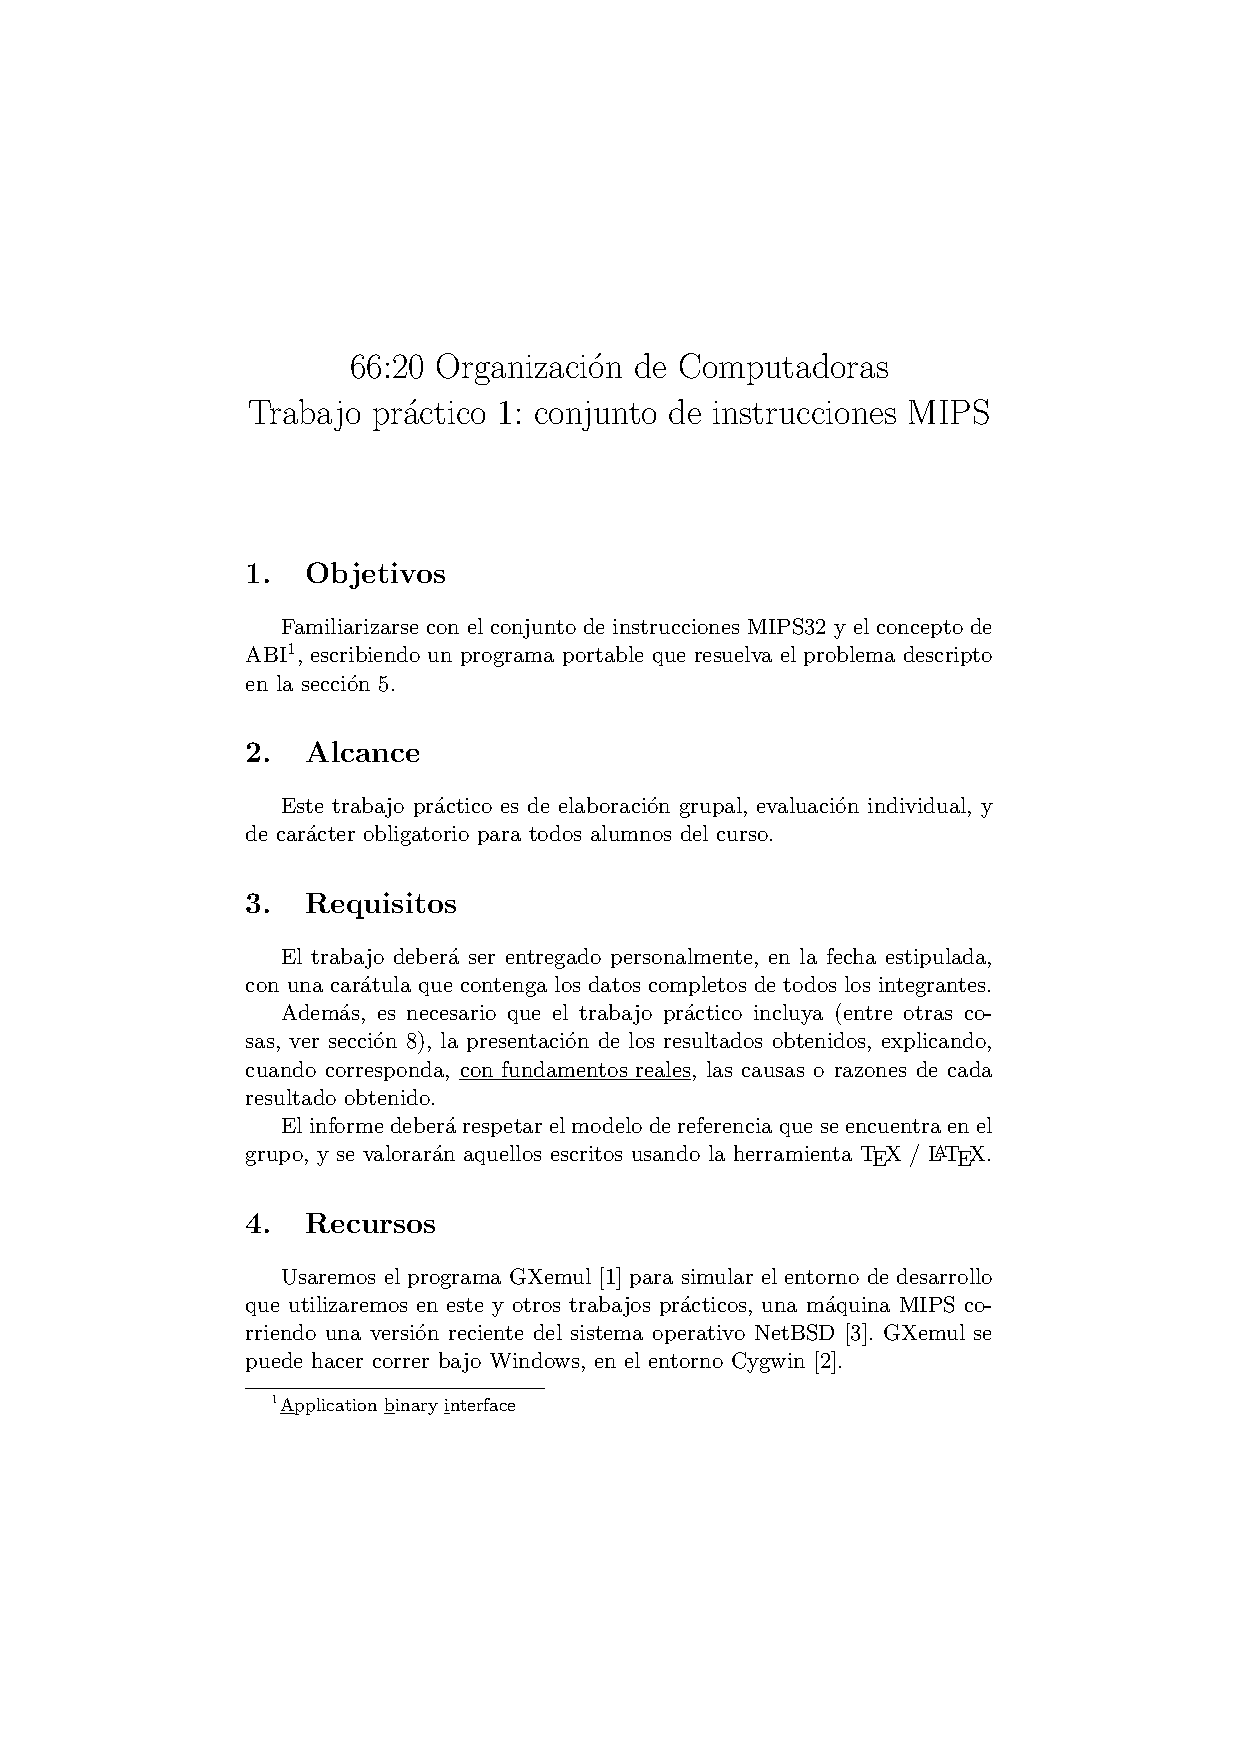
\includegraphics[scale=1, page = 1, clip, trim=1.5in 36mm 20mm 35mm]{files/enunciado.pdf}
	\end{figure}
	
	\newpage
	\begin{figure}[H]
		\centering
		\includegraphics[scale=1, page = 2, clip, trim=1.5in 36mm 20mm 20mm]{files/enunciado.pdf}
	\end{figure}
	
	\newpage
	\begin{figure}[H]
		\centering
		\includegraphics[scale=1, page = 3, clip, trim=1.5in 36mm 20mm 20mm]{files/enunciado.pdf}
	\end{figure}
	
	\newpage
	\begin{figure}[H]
		\centering
		\includegraphics[scale=1, page = 4, clip, trim=1.5in 36mm 20mm 20mm]{files/enunciado.pdf}
	\end{figure}
	
	\newpage
	\begin{figure}[H]
		\centering
		\includegraphics[scale=1, page = 5, clip, trim=1.5in 36mm 20mm 20mm]{files/enunciado.pdf}
	\end{figure}
	
	\section{Desarrollo}
	\
	
		El programa puede tomar opciones de entrada para indicar el tipo de ordenamiento (alfabético o numérico) y argumentos que designan la salida y el archivo a ordenar.
		
	\subsection{Implementación}
		
		Los errores se definen como cadenas de caracteres constantes. Los mensajes de error se llaman con una función a la que se le pasa el mensaje a mostrar y el número que le corresponde al error.
		
		Las invocaciones a la línea de comandos (como el pedido de versión o de ayuda) también se guardan en cadenas. El tipo de mensaje a mostrar es pasado a la función que los visualiza.
		
		El programa podrá tomar sólo un parámetro, en caso que se desee acceder a la ayuda o a la versión, y un máximo de cuatro cuando se quiera ordenar un archivo. El primero de estos será el tipo de ordenamiento, que se considerará alfabético por defecto, por lo que este parámetro puede no estar; luego vendrá el output (\texttt{-o} o \texttt{--output}); el tercero será el archivo donde se escribirá el resultado del ordenamiento (\texttt{stdout} en caso de que se ingrese \texttt{-}); y por último el archivo a ordenar. Ingresar estos parámetros en cualquier otro orden resultará en un mensaje de error.
		
		Al inicio de la función \texttt{main} se verificarán los argumentos ingresados para ver si coinciden con las opciones requeridas para que el programa pueda responder de acuerdo con el comportamiento elegido.
		
		Se decidió por implementar una versión \textit{in place} del algoritmo Quicksort, por cuestiones de simplicidad y para mayor legibilidad el código. Ésta diferencia el tipo de ordenamiento que se hará en un método de ordenamiento general, lo cual se logra con un entero identificador: si vale 1, el ordenamiento es numérico; para cualquier otro valor se realizará un ordenamiento alfabético. En el primer caso se utilizará una función atoi para pasar las cadenas de caracteres a números enteros mientras que en el otro caso se compararán las cadenas entre sí. 
		
		Se elegió cambiar el nombre de la función qsort puesto que esta se encuentra reservada por C. Se llamará orgaqsort a la función implementada en C, y orgaqsortassembly a su contraparte en assembly.
		
		El comando utilizado para compilar el programa será \texttt{gcc -Wall -o qsort qsort.c orgaqsortassembly.s} 
	\subsubsection{Diagramas de stack}
		A continuación se muestran los diagramas de stack de las diferentes funciones del archivo assembly.
		\begin{table}
			\begin{center}
				\begin{tabular}{|C{2cm}|C{2cm}|}
					\hline
					\multirow{4}{*}{\textbf{SRA}} & padding\\\cline{2-2}
					&ra\\\cline{2-2}
					&fp\\\cline{2-2}
					&gp\\
					\hline
					\multirow{4}{*}{\textbf{LTA}} & fin\\\cline{2-2}
					&inicio\\\cline{2-2}
					&der\\\cline{2-2}
					&izq\\
					\hline
					\multirow{4}{*}{\textbf{ABA}} & \\\cline{2-2}
					&a2\\\cline{2-2}
					&a1\\\cline{2-2}
					&a0\\
					\hline
				\end{tabular}
			\caption{Diagrama de stack de la función \texttt{orgaqsortasembly}}
			\label{tab:Figura1}
			\end{center}
		\end{table}
		\begin{table}
			\begin{center}
				\begin{tabular}{|C{2cm}|C{2cm}|}
					\hline
					\multirow{4}{*}{\textbf{SRA}} & padding\\\cline{2-2}
					&ra\\\cline{2-2}
					&fp\\\cline{2-2}
					&gp\\
					\hline
					\multirow{4}{*}{\textbf{ABA}} & \\\cline{2-2}
					&\\\cline{2-2}
					&\\\cline{2-2}
					&a0\\
					\hline
				\end{tabular}
			\caption{Diagrama de stack de la función \texttt{comparar}}
			\label{tab:Figura1}
			\end{center}
		\end{table}
		\begin{table}
			\begin{center}
				\begin{tabular}{|C{2cm}|C{2cm}|}
					\hline
					\multirow{2}{*}{\textbf{SRA}}
					&fp\\\cline{2-2}
					&gp\\
					\hline
				\end{tabular}
			\caption{Diagrama de stack de la función \texttt{atoi}}
			\label{tab:Figura1}
			\end{center}
		\end{table}
	\subsection{Pruebas}
	
	\subsubsection{Entradas incorrectas}
	Ingresando sólo el nombre del programa ejecutable:
	\begin{verbatim}
$ ./qsort
qsort: La cantidad de parametros no es la correcta.
Intente 'qsort -h' para mas informacion
	\end{verbatim}
	Ingresando un argumento inválido:
	\begin{verbatim}
$ ./qsort -w
qsort: La combinacion de parametros no es la correcta.
Intente 'qsort -h' para mas informacion
	\end{verbatim}
	Ingresando más argumentos de los necesarios:
	\begin{verbatim}
$ ./qsort f f f f f
qsort: La cantidad de parametros no es la correcta.
Intente 'qsort -h' para mas informacion
	\end{verbatim}
	Ingresando un archivo que no existe:
	\begin{verbatim}
$ ./qsort -o - numbers.txt
El archivo que quiere ordenar no existe
	\end{verbatim}
	Ingresando el orden incorrecto de parámetros (primero \texttt{-o} y luego \texttt{-n}):
	\begin{verbatim}
$ ./qsort -o -n - numeros.txt
qsort: La combinacion de parametros no es la correcta.
Intente 'qsort -h' para mas informacion
	\end{verbatim}
Aquí detecta que la opción de ordenamiento alfabético tiene argumentos de más.
	
	
	
	\subsubsection{Ordenando líneas}
Ingresando un archivo para ordenar alfabéticamente:
	\begin{verbatim}
$ ./qsort -o - zeta.txt
zzzzzzzzzzzz a
zzzzzzzzzzzz b
zzzzzzzzzzzz sabia que Asuntos Internos le tendia una trampa
	\end{verbatim}
	
	\begin{verbatim}
$ ./qsort -o - text1.txt
 aaaaaaa
aaaaaaa
aaaaaaa a
aaaaaaa b
aaaaaaaaaaaaaaaaaaaaaaaaaaaaaaaaaaaaaaaaaaaaaaaaaaaaaaaaaaaaaa
aaaaaaaaaaaaaaaaaaaaaaaaaaaaaaaaaaaaaaaaaaaaaaaaaaaaaaaaaaaaaa
aaaaaaaaaaaaaaaaaaaaaaaaaaaaaaaaaaaaaaaaaaaaaaaaaaaaaaaaaaaaaa
aaaaaaaaaaaaaaaaaaaaaaaaaaaaaaaaaaaaaaaaaaaaaaaaaaaaaa
hola 

que 
tal 

	\end{verbatim}
	Ingresando el nombre del archivo que se desea para salida de un ordenamiento alfabético:
	\begin{verbatim}
$ ./qsort -o orden_alfabetico.txt numeros.txt
	\end{verbatim}
	Se genera un archivo con el nombre \texttt{orden\_alfabetico.txt} que contiene las palabras de \texttt{numeros.txt} en orden alfabético.
	\begin{verbatim}
$ cat orden_alfabetico.txt
1
10
2
3
4
5
6
7
8
9
	\end{verbatim}
Ingresando un archivo para ordenar numéricamente:
		
	\begin{verbatim}
$ ./qsort -n -o - numeros.txt
1
2
3
4
5
6
7
8
9
10
	\end{verbatim}
	Ingresando el nombre del archivo que se desea para salida de un ordenamiento numérico:
	\begin{verbatim}
$ ./qsort -n -o orden_numerico.txt zeta.txt
	\end{verbatim}
	Se genera un archivo con el nombre \texttt{orden\_alfabetico.txt} que contiene las palabras de \texttt{zeta.txt} en orden numérico.
	\begin{verbatim}
$ cat orden_numerico.txt
zzzzzzzzzzzz sabia que Asuntos Internos le tendia una trampa
zzzzzzzzzzzz a
zzzzzzzzzzzz b
	\end{verbatim}
	Por cuestiones de espacio no se muestran los resultados de correr el programa con los archivos \texttt{alice.txt} y \texttt{quijote.txt}.
	
	\section{Conclusiones}
	
	La realización de este trabajo resultó de mucha utilidad para entender como funcionan las herramientas usadas, como el emulador y el lenguaje, algo que se presentó dificil en un principio. También contribuyó para incorporar las convenciones usadas para trabajar con a arquitectura MIPS.
	Por otra parte, permitió aprender a programar en lenguaje ensamblador, prestándole atención a los detalles y valiéndose de las estructuras generadas por las funciones, como la pila, para almacenar los parámetros cuyo valor se quiere seguir a lo largo de la ejecución de esa función en particular. Sumado a esto, sirvió para comprender cómo combinar archivos en C y archivos en lenguaje assembly, cosa inédita hasta ese momento.
	Sacamos del trabajo buenas prácticas, como lo son el probar las funciones del codigo assembly por separado para luego incorporarlas, ya que una vez que está todo junto se hace mas complejo; y el uso del debugger tanto para solucionar los problemas que pudiera tener el programa como para realizar el seguimiento del código ejecutado.
	
	Se entregan dos scripts. Uno en C, con una implementacion de qsort en C y otras funciones necesarias; y uno en assembly sólo con la funciones \texttt{qsort}, \texttt{comparar} y \texttt{atoi}.
\end{document}
